This section should describe the overall structure of your software system. Think of it as the strategy for how you will build the system. An architectural "layer" is the top-level logical view, or an abstraction, of your design. Layers should be composed of related elements of similar capabilities, and should be highly independent of other layers, but should have very clearly defined interfaces and interactions with other layers. Each layer should be identified individually and should be unique as to its function and purpose within the system. This section should also contain the high-level block diagram of the layers, as shown in the example below, as well as detailed descriptions of the functions of each layer.

\begin{figure}[h!]
	\centering
 	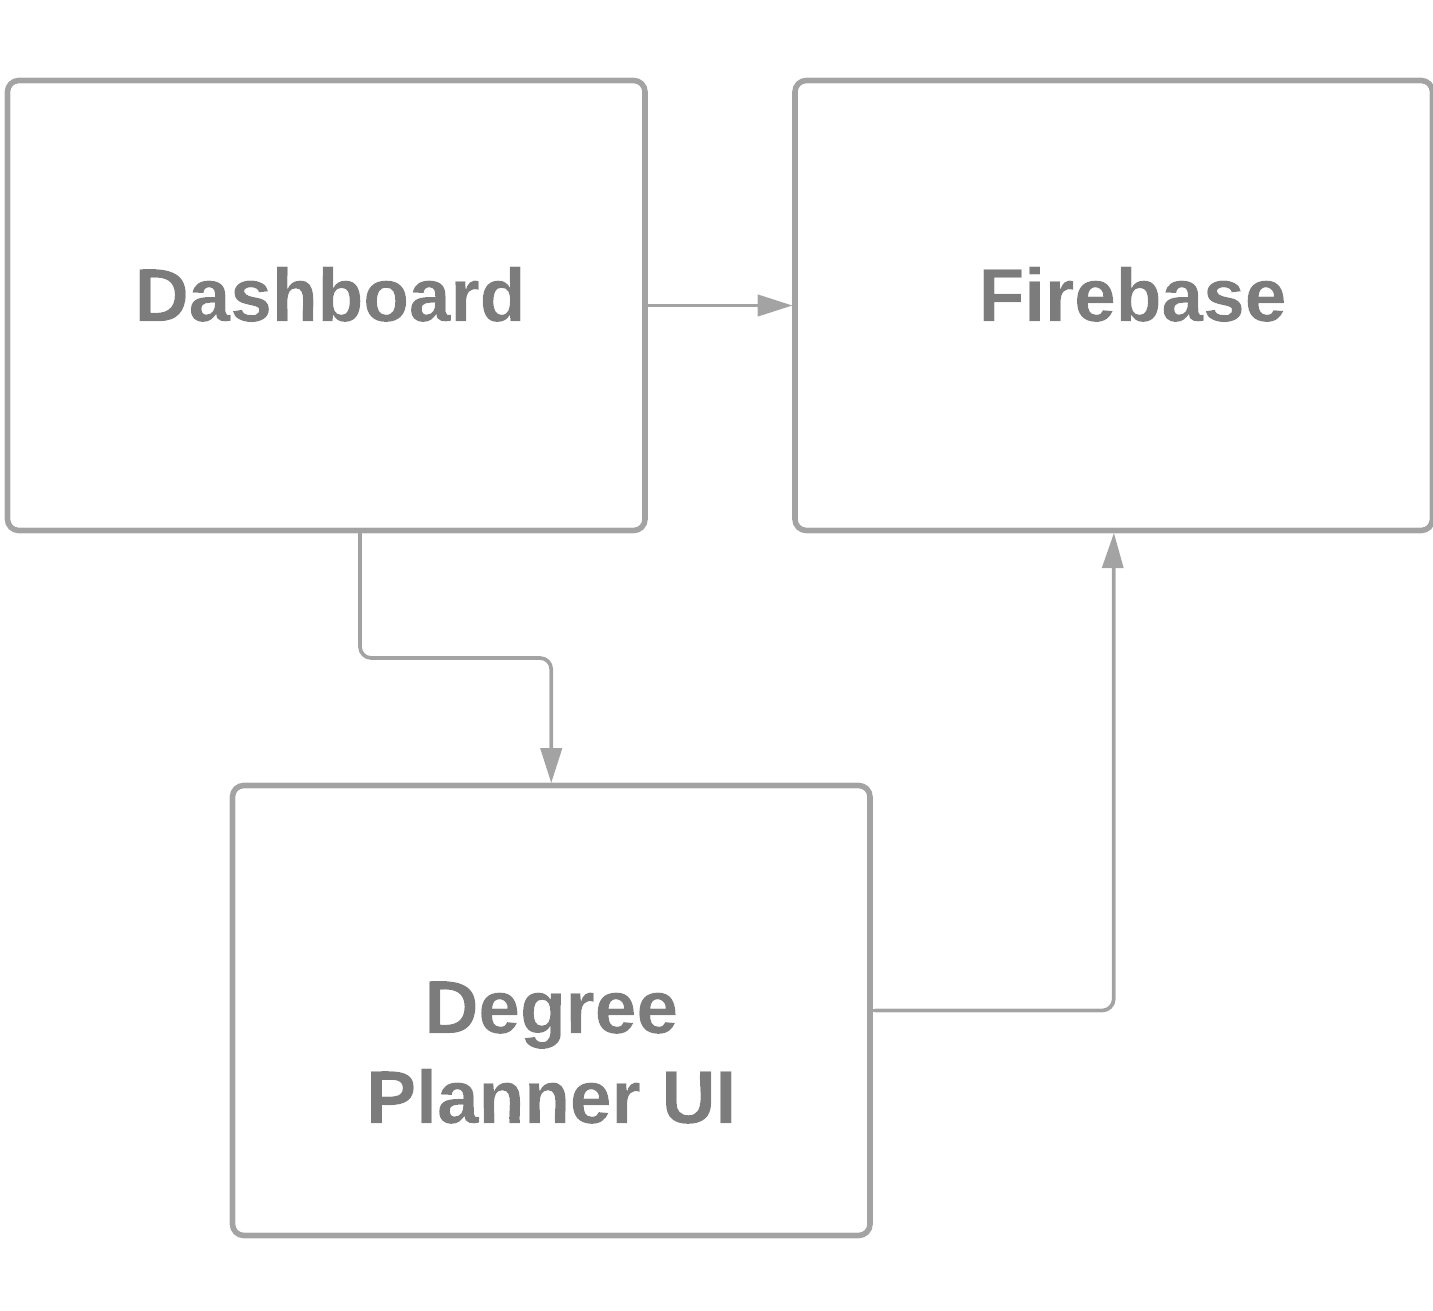
\includegraphics[width=0.60\textwidth]{images/system_overview_pic}
 \caption{A simple architectural layer diagram}
\end{figure}

\subsection{Degree Planner UI Description}
Each layer should be described separately in detail. Descriptions should include the features, functions, critical interfaces and interactions of the layer. The description should clearly define the services that the layer provides. Also include any conventions that your team will use in describing the structure: naming conventions for layers, subsystems, modules, and data flows; interface specifications; how layers and subsystems are defined; etc.

    The degree planner UI will have features allowing users to easily select and interact with their degree plans. It will allow users to select classes, display information, and give the user access to navigate between the Dashboard and the degree planning section. The UI will interact with Firebase when the student selects classes. It will get the data from Firebase and bring it to the UI layer. Once the UI has the data, it will then display the data to the users. The UI will also allow the users to navigate between screens and give them access to switch to the Dashboard screen. We will call this the Degree Planner UI layer.

    

    

\subsection{Firebase Description}
Each layer should be described separately in detail. Descriptions should include the features, functions, critical interfaces and interactions of the layer. The description should clearly define the services that the layer provides. Also include any conventions that your team will use in describing the structure: naming conventions for layers, subsystems, modules, and data flows; interface specifications; how layers and subsystems are defined; etc.

    The firebase layer has features such as keeping data, authentication, and sending data. When a user selects classes the UI layer will request the data from firebase. Firebase will

\subsection{Dashboard Description}
Each layer should be described separately in detail. Descriptions should include the features, functions, critical interfaces and interactions of the layer. The description should clearly define the services that the layer provides. Also include any conventions that your team will use in describing the structure: naming conventions for layers, subsystems, modules, and data flows; interface specifications; how layers and subsystems are defined; etc. 

    The dashboard layer of the degree planner will have a link to the degree planner, it will allow the user to sign in and out of their account, and it will let the user see the flowchart of their major. The user will be able to make an account in the dashboard. They will give their information and be able to make an account. Once their account is made, their data will be sent over and stored in firebase. They can then sign in and out with the use of the dashboard and everytime they sign in and out. The authentication will be handled through firebase. In the dashboard there will also be the option for the user to click on a link to see the flowchart of their major. This layer will be called the dashboard layer. 